% !TeX root = ../../Parte3.tex
\secmeme{js/semicolon}
\section{Primi passi}
\begin{frame}[fragile]{Messaggi}\transfade\centering
  \begin{enumerate}
    \item Finestre di dialogo (per l'utente):
      \begin{columns}
        \begin{column}{.5\textwidth}
          \begin{minted}{js}
alert("Ciao!");
          \end{minted}
        \end{column}
        \begin{column}{.5\textwidth}\centering
          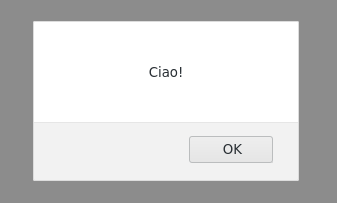
\includegraphics[width=.6\columnwidth]{img/alert}
        \end{column}
      \end{columns}
    \item Stampa nella consolle (per debug):
    \begin{columns}
      \begin{column}{.5\textwidth}
        \begin{minted}{js}
console.log("Ciao!");
          \end{minted}
        \end{column}
        \begin{column}{.5\textwidth}
          \begin{minted}{sh}
Ciao!
>
          \end{minted}
        \end{column}
      \end{columns}
  \end{enumerate}
\end{frame}

\begin{frame}[fragile]{Variabili}\transfade\centering
  \begin{minted}{js}
// Dichiarazione
var pippo; // variabile globale: sconsigliato usarle
let pluto; // variabile locale

// Assegnamento
pluto = 20;

// Dichiarazione con inizializzazione
let paperino = "duck";

// Costanti (obbligatria inizializzazione)
const TOPOLINO = 1.5;

// Utilizzo
pluto = 7 * (TOPOLINO + pluto % 6) / 2**3 - 1;
//      7 · ( 1.5     +  20 mod 6) ÷  2³  - 1
alert(pluto);  // 2.0625
  \end{minted}
  \pause
  \alert{Attenzione!} Usare varibili non dichiarate non da errore, ma non va fatto!!!\\
  Inserire nella prima riga \mintjs[bgcolor=mintbg]{"use strict";} per evitare questo ed altri errori.\\
\end{frame}

\begin{frame}[fragile]{Stringhe}\transfade\centering
  \begin{minted}[fontsize=\normalsize]{js}
let a = "Questa è una stringa";
let b = 'Questa è una stringa';
let c = 'Questa è una "stringa"';

let pippo = 15;
let d = "Il totale è " + pippo + " euro"; // concatenazione
let e = `Il totale è ${pippo} euro`; // interpolazione
  \end{minted}
  \bigskip
  Come scrivere l'accento grave (\texttt{\`}):
  \begin{description}
    \item[Linux] \texttt{AltGr} + \texttt{\'}
    \item[Windows\footnote{Dal tastierino numerico.}] \texttt{Alt} + \texttt{96}
    \item[macOS\footnote{In alcuni computer potrebbe essere necessario digitare uno spazio dopo questa combinazione di tasti.}] \texttt{AltGr} + \texttt{\textbackslash} o \texttt{AltGr} + \texttt{9}
  \end{description}
\end{frame}